%!TEX root = main.tex
\chapter{Future Work}

This chapter gives recommendations for the future of the TaleBlazer Analytics system, including new features and technical improvements. 

\section{Data Visualizations}

Currently, the analytics site only provides a tabular view for analytics data. Although this data provides useful information for analytics users, it can be difficult to get a high-level understanding of the statistics quickly. As a result, it would be useful to implement visualizations of the analytics data. 

Data visualizations would allow users to quickly interpret and draw conclusions from analytics data. This feature would improve the usability of the site and allow users to focus more on the overall results of the data, rather than having to interpret the results from the tabular data. For example, Figure \ref{fig:num_completed_viz} shows a visualization detailing how many players played specific versions of a game over a week. 

\begin{figure}[htb]
	\center{
			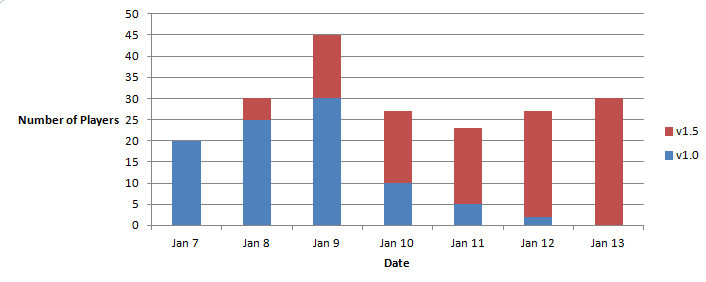
\includegraphics[width=\textwidth]
				{figures/num_completed_viz.png}
			}
	\caption[Example Data Visualization]{\label{fig:num_completed_viz} Distribution of Total Players by Game Version, over a week}
\end{figure}

The TaleBlazer Analytics system was built to accommodate visualizations from the start of its development. The relevant data is already provided in JSON via the same API call that allows pages to retrieve their relevant analytics data. Visualization implementation is easily accomplished via D3.js, a popular JavaScript visualization library.

\section{Authentication/Authorization}

In order to restrict users to view only data for their games, it is necessary to implement an authentication and authorization system. Although a simple login and permission system could be set up for TaleBlazer Analytics quickly, it is important to build a system that allows users to use their same credentials from TaleBlazer Server. This would avoid the problem of having multiple credentials for the two services. This system was delayed in order to prioritize the data collection and analysis features of TaleBlazer Analytics.

A way to implement this would be for the analytics server to utilize the same session information currently used by TaleBlazer Server. A simple solution would be for TaleBlazer Server to use database-backed sessions, which would allow the analytics server to access the session data directly.

A more extensive solution would be to implement OAuth2, which is a protocol for security authentication and authorization. This solution would involve implementing OAuth into TaleBlazer Server or deploying a separate server solely responsible for authentication and authorization. Plugins for CakePHP currently exist for enabling this functionality. 

\section{Improved Statistic Calculation}

Statistics are currently calculated every time that a request to an analytics page is made. Although the statistic calculations are optimized to offload the majority of the work to the database, the calculation times may take longer as more data is collected. Two options for mitigating this issue are to perform progressive calculation and to store the calculation results using an in-memory cache. 

Progressive calculation means that statistics are calculated and stored separately as the data is received from TaleBlazer Mobile. As a result, statistics are already available when requested by a page and so the computational overhead per request is significantly decreased. 

An in-memory cache would solve the issue of unnecessary recalculation. In-memory caches, such as Redis and Memcached, allow incredibly fast access to data because the data is stored in RAM. Cached data can be expired and removed based on conditions set by the developer, such as newly arrived data. Storing the results of calculations in an in-memory cache would solve the issue of unnecessary recalculations. A typical request would consult with the cache first to see if the statistics are already stored. If still valid, the request would return the statistics. Otherwise, the server would perform the calculation as normal.

\section{Code Improvements}

Future technical improvements to the server codebase involve creating a Service layer to consolidate common model-related functions and the use of the \texttt{async} JavaScript library for improving the readability of asynchronous code. 

Currently, the controllers for each API contain code to modify, retrieve, and save models as required by the API. A Service layer would remove model-specific code from controllers and place them into modules known as Services. Each service would be responsible for handling common functions related to a model. For example, a Device Service would handle common device registration tasks and duplicate device checks. Ultimately, this would allow controllers to focus on validating inputs and responding to requests. The majority of the work with models would then live in the corresponding service.

The \texttt{async} JavaScript library provides a set of utility functions which handle common asynchronous tasks. The asynchronous nature of JavaScript code results in multiple levels of callback functions, which is often difficult to read and modify. The async library solves this issue by providing a powerful set of utility functions that improve the readability of the code. Compare the readability of the two functions in Listing \ref{lst:async}, which perform the same tasks. 

\medskip
\begin{lstlisting}[caption={[Typical Nested Code vs \texttt{async} library]Comparison between normal callback code and \texttt{async} code}, label={lst:async}]
// Nested callbacks
// Each function waits on the results of the previous one before continuing
performAction1(function(){
	performAction2(function() {
		performAction3(function() {
			// and so on...
			})
		})
	})

// Callbacks using async library
// Results of each function are passed to the other using the next parameter
// When all are executed, the finalCallback is executed
async.waterfall([
		performAction1(next), 
		performAction2(next),
		performAction3(next)
	], finalCallback)
});
\end{lstlisting}









